% demo.tex
%
% Enjoy, evolve, and share!
%
% Compile it as follows:
%   latexmk
%
% Check file `dithesis.cls' for other configuration options.
%
\documentclass[ack,preface]{dithesis}

%\usepackage{graphicx}

%%%%%%%%%%%%%%%%%%%%%%%%%%%%%%%%%%%%%%%%%%%%%%%%%%%%%%%%%%%%%%%%%%%%%%%%%%%%%%%
%%%%%%%%%%%%%%%%%%%% User-specific package inclusions %%%%%%%%%%%%%%%%%%%%%%%%%
%%%%%%%%%%%%%%%%%%%%%%%%%%%%%%%%%%%%%%%%%%%%%%%%%%%%%%%%%%%%%%%%%%%%%%%%%%%%%%%
\usepackage{booktabs}
\usepackage{hyperref}
\usepackage{lipsum}
\usepackage{enumerate}
\usepackage{amsmath}
\usepackage{amssymb}
\hypersetup{
    unicode=true,                     % non-Latin characters in bookmarks
    pdffitwindow=true,                % page fit to window when opened
    pdfnewwindow=true,                % links in new window
    pdfkeywords={},                   % list of keywords
    colorlinks=true,                  % false: boxed links; true: colored links
    linkcolor=black,                  % color of internal links
    citecolor=black,                  % color of links to bibliography
    filecolor=black,                  % color of file links
    urlcolor=black,                   % color of external links
    pdftitle={},                      % title
    pdfauthor={},                     % author
    pdfsubject={}                     % subject of the document
}
%%%%%%%%%%%%%%%%%%%%%%%%%%%%%%%%%%%%%%%%%%%%%%%%%%%%%%%%%%%%%%%%%%%%%%%%%%%%%%%
%%%%%%%%%%%%%%%%%%%% User-specific package inclusions %%%%%%%%%%%%%%%%%%%%%%%%%
%%%%%%%%%%%%%%%%%%%%%%%%%%%%%%%%%%%%%%%%%%%%%%%%%%%%%%%%%%%%%%%%%%%%%%%%%%%%%%%


%%%%%%%%%%%%%%%%%%%%%%%%%%%%%%%%%%%%%%%%%%%%%%%%%%%%%%%%%%%%%%%%%%%%%%%%%%%%%%%
%%%%%%%%%%%%%%%%%%%%%% User-specific configuration %%%%%%%%%%%%%%%%%%%%%%%%%%%%
%%%%%%%%%%%%%%%%%%%%%%%%%%%%%%%%%%%%%%%%%%%%%%%%%%%%%%%%%%%%%%%%%%%%%%%%%%%%%%%
%%%%%%%%%%%%%%%%%%%%%%%%%%%%%%%%%%%%%%%%%%%%%%%%%%%%%%%%%%%%%%%%%%%%%%%%%%%%%%%
%%%%%%%%%%%%%%%%%%%%%% User-specific configuration %%%%%%%%%%%%%%%%%%%%%%%%%%%%
%%%%%%%%%%%%%%%%%%%%%%%%%%%%%%%%%%%%%%%%%%%%%%%%%%%%%%%%%%%%%%%%%%%%%%%%%%%%%%%


%%%%%%%%%%%%%%%%%%%%%%%%%%%%%%%%%%%%%%%%%%%%%%%%%%%%%%%%%%%%%%%%%%%%%%%%%%%%%%%
%%%%%%%%%%%%%%%%%%%%%%%%%%% Required Metadata %%%%%%%%%%%%%%%%%%%%%%%%%%%%%%%%%
%%%%%%%%%%%%%%%%%%%%%%%%%%%%%%%%%%%%%%%%%%%%%%%%%%%%%%%%%%%%%%%%%%%%%%%%%%%%%%%
%
% First name, last name
%
\authorFirstGr{Καλλιόπη}
\authorFirstAbrGr{Κ.} % abbreviation of first name
\authorMiddleGr{Π.}   % abbreviation of father's first name
\authorLastGr{Κωστοπούλου}
\authorFirstEn{Calliope}
\authorFirstAbrEn{C.}
\authorMiddleEn{P.}
\authorLastEn{Kostopoulou}
\authorSn{1115201200084}

%
% The title of the thesis
%
\titleEn{Recursive Function Definitions in Static Dataflow Graphs and their implementation in TensorFlow}
\titleGr{Ορισμοί αναδρομικών συναρτήσεων σε στατικούς dataflow γράφους και η υλοποίηση τους στο TensorFlow}

%
% Month followed by Year
%
\dateGr{ΣΕΠΤΕΜΒΡΙΟΣ 2018}
\dateEn{SEPTEMBER 2018}

%
% Supervisor(s) info
%
\supervisorGr{Άγγελος Χαραλαμπίδης}{Ερευνητής ΕΚΕΦΕ Δημόκριτος}
\supervisorGr{Παναγιώτης Ροντογιάννης}{Καθηγητής ΕΚΠΑ}
\supervisorEn{Angelos Charalambidis}{Researcher NCSR Demokritos}
\supervisorEn{Panos Rondogiannis}{Professor NKUA}
%
% Abstract, synopsis, inscription, ack, and preface pages.
%
\abstractEn{
Dataflow is  an alternative programming paradigm which proposes that every computation is represented as a graph.
This representation could be thought of, perhaps, as an enhanced version of the classic one because it contains information about both the tasks that need to be carried out and the underlying data dependencies. A dataflow execution model can use this information to execute all the non-dependent code segments out of order and in parallel which can, theoretically, increase the degree of parallelism to the maximum possible level. Dataflow's potential for immense parallelism/distribution has made this model extremely popular in the Machine Learning community where there is  a great number of new dataflow-based frameworks that have been recently developed for this purpose. Embedding dynamic control flow features,  such as if-else constructs, iteration or even recursive function definitions, inside those dataflow graphs, is extremely needed in this field for expressing complex computations and certain kinds of neural networks, however, it is not as trivial as we would like it to be. Two main approaches have been suggested as a solution, in the dataflow community, so far. The first one (dynamic) leads to the creation of graphs that transform themselves on demand, during runtime, while the second one (static) proposes the creation of static, non-transforming graphs that retain their initial form throughout the whole execution. The second approach is quite more profound, as it needs the introduction of a concept called “tagging” in order to work. The various dataflow systems that have recently emerged, follow either the first or the second approach when they need to support such dynamic control flow features. None of them, however, to the best of our knowledge, does follow the second approach when it comes to supporting recursive function definitions, as the tagging mechanism that needs to be employed is considered to be rather complex and possibly is avoided. The subject of this thesis, is the proposal of a systematic way to embed recursive function definitions in static dataflow graphs, based on ideas expressed during the extended research that already has been made regarding this topic, at the past.  A great part of this thesis, has also been the implementation of these ideas in a famous, rapidly growing, dataflow-based framework called TensorFlow, which was made by Google for Machine Learning purposes.
}
\abstractGr{
\begin{greek}
Το Dataflow είναι ένα εναλλακτικό μοντέλο προγραμματισμού στο οποίο κάθε υπολογισμός αναπαρίσταται σαν ένας γράφος. Αυτή η αναπαράσταση μπορεί να θεωρηθεί, ενδεχομένως, σαν μια ενισχυμένη έκδοση της κλασικής/συμβατικής αναπαράστασης προγραμμάτων επειδή περιέχει πληροφορίες τόσο για τους υπολογισμούς που πρέπει να πραγματοποιηθούν όσο και για τις αλληλοεξαρτήσεις των δεδομένων. Ένα dataflow μοντέλο εκτέλεσης μπορεί να χρησιμοποιήσει αυτές τις πληροφορίες για να εκτελέσει όλα τα "ανεξάρτητα" τμήματα κώδικα  παράλληλα κάτι το οποίο μπορεί να αυξήσει, θεωρητικά, το βαθμό παραλληλίας στο μέγιστο δυνατό επίπεδο. Η δυνατότητα του μοντέλου αυτού για μια τόσο μεγάλη, ενδεχόμενη παραλληλία το έχει καταστήσει ιδιαίτερα διάσημο στην κοινότητα του Machine Learning όπου έχει δημιουργηθεί ένα μεγάλο πλήθος από dataflow συστήματα συγκεκριμένα για αυτόν τον σκοπό.
Η ενσωμάτωση χαρακτηριστικών δυναμικής ροής ελέγχου όπως  η επανάληψη, η αναδρομή ή η εκτέλεση υπο συνθήκη σε αυτούς τους γράφους είναι εξαιρετικά χρήσιμη στον τομέα του Machine Learning, έτσι ώστε να μπορούν να εκφράζονται εύκολα πολύπλοκοι υπολογισμοι καθώς και συγκεκριμένα είδη νευρωνικών δικτύων, ωστόσο δε γίνεται με τόσο προφανή τρόπο όσο θα θέλαμε. Δύο βασικές προσεγγίσεις έχουν προταθεί σαν λύση από την dataflow κοινότητα, μέχρι στιγμής. Η πρώτη (δυναμική) προκαλεί τη δημιουργία γράφων που μετασχηματίζονται, κατ' απαίτηση, κατα τη διάρκεια της εκτέλεσης, ενώ η δεύτερη (στατική) προτείνει τη δημιουργία στατικών γράφων που διατηρούν την αρχική τους μορφή κατα τη διάρκεια όλης της εκτέλεσης. Η δεύτερη προσέγγιση είναι ελαφρώς πιο σύνθετη μιας και απαιτεί να εισάγουμε την έννοια του "tagging" ώστε να επιτευχθεί. Τα διάφορα dataflow συστήματα που έχουν αναπτυχθεί εώς τώρα, ακολουθούν είτε την πρώτη είτε την δεύτερη προσέγγιση, όταν χρειάζεται να υποστηρίξουν τέτοια χαρακτηριστικά δυναμικής ροής ελέγχου. Κανένα, ωστόσο, απ' όσο γνωρίζουμε, δεν ακολουθεί την δεύτερη προσέγγιση όταν πρόκειται να υποοστηρίξει ορισμούς αναδρομικών συναρτήσεων, διότι ο "tagging" μηχανισμός που χρειάζεται να υλοποιηθεί θεωρείται περίπλοκος και πιθανώς αποφεύγεται. Το θέμα αυτής της πτυχιακής εργασίας είναι η πρόταση μιας συστηματικής μεθόδου για την ενσωμάτωση ορισμών αναδρομικών συναρτήσεων σε στατικούς dataflow γράφους, βασισμένη στην εκτεταμένη έρευνα που έχει ήδη γίνει στο παρελθόν όσον αφορά σε αυτό το θέμα. Ένα μεγάλο μέρος της εργασίας αυτής ήταν εκτός των άλλων και η υλοποίηση αυτών των ιδεών σε ένα διάσημο, ταχέως διευρυνόμενο dataflow σύστημα που ονομάζεται TensorFlow και δημιουργήθηκε από την Google για τους σκοπούς του Machine Learning.
\end{greek}
}
\acksEn{
I would like to thank both Panos Rondogiannis and Angelos Charalambidis for giving me the chance to work on a challenging project and for coming up with this interesting subject on the first place.

I am especially grateful to Angelos who has been helping  me for the last few months and making me consider him more of a teammate than a simple supervisor.
His special psychic abilities, that make him come up with accurate solutions, provided me with great comfort when I’d see my intuition leading me to all the wrong places.
}
\prefaceEn{
The objective of the task that was initially proposed to me, as a subject for this bachelor thesis, was to investigate ways of implementing and integrating recursion in TensorFlow by creating dataflow graphs that are static and therefore, retain their initial form at runtime, opposite to Google’s approach, which relies on graphs that expand themselves during execution. This work is meant to demonstrate that the idea for producing static dataflow graphs from recursive function definitions, expressed in this \cite{Rondogiannis:1997} prior research work can be easily applied to data driven models and still be feasible. Another huge motivation, was the fact that recursion, as a feature in dataflow systems, is highly desired by people who are active in the machine learning field, as the additional expressiveness possibly leads to superior performance results in cases of recursive neural networks. A great amount of time, during my engagement with this project, was dedicated to studying the dataflow programming paradigm in general and an even greater one was spent on digging around TensorFlow’s core code for acquiring the necessary knowledge as much as the confidence to add the appropriate code and implement the aforementioned ideas.
}

\inscriptionEn{\emph{}}

%
% Subject area and keywords
%
\subjectAreaGr{Μοντέλο Ροής Δεδομένων}
\subjectAreaEn{Dataflow Model}
\keywordsGr{dataflow, tensorflow, στατικοί dataflow γράφοι, αναδρομικοί ορισμοί συναρτήσεων, αναδρομή, κατανεμημένα συστήματα, δυναμική ροή δεδομένων}
\keywordsEn{dataflow, tensorflow, static dataflow graphs, recursive function definitions, recursion, distributed computing, dynamic control flow}

%
% Set the .bib file containing your paper publications (leave the extension out)
%
% This is optional, but it should be specified when option 'lop' is passed to
% the document class.
%
% Then, inside the document environment, you may use the command '\nocitelop' to
% site your papers, as you would traditionally do with the commands '\cite' or
% '\nocite'.
%
% The papers are printed in reverse chronological order.
%
%\lopfile{mypapers/pubs}
%%%%%%%%%%%%%%%%%%%%%%%%%%%%%%%%%%%%%%%%%%%%%%%%%%%%%%%%%%%%%%%%%%%%%%%%%%%%%%%
%%%%%%%%%%%%%%%%%%%%%%%%%%% Required Metadata %%%%%%%%%%%%%%%%%%%%%%%%%%%%%%%%%
%%%%%%%%%%%%%%%%%%%%%%%%%%%%%%%%%%%%%%%%%%%%%%%%%%%%%%%%%%%%%%%%%%%%%%%%%%%%%%%

\begin{document}

\frontmatter

\mainmatter

% add main chapters (should be given in capital letters)
\chapter{INTRODUCTION}
    \section{Main Concept}
	In the conventional, von Neumann model, a program is represented as a sequence of instructions, whose order of execution is implicitly described by the programmer.
The execution of a code segment, representing a recursive function, in the above architecture, is handled with the help of a register, called program counter, whose value always points to the address of the instruction that is meant to be executed next (instruction pointer). This code segment is supposed to be executed every time the recursive function calls itself which is a decision that, in most cases, can only be made at runtime (dynamic control flow). Whenever such calls occur, the program counter updates its value appropriately so that the execution jumps to the correct instruction, re-entering the same code segment again and again. This way the executable code contains once the code of the recursive function which is re-computed whenever necessary. An alternative approach to that, however, would be to modify the executable code at runtime  and handle each recursive call by inserting the corresponding code-segment dynamically to the default, following address, where the PC is normally supposed to point next (PC+4 in most cases). Every recursive call would now cause the expansion of the executable code and no jumps would occur during the execution.
From now on, we will refer to those two approaches as "static" and "dynamic", respectively.

As opposed to the model described above, dataflow programming paradigm adopts a data driven computational model which allows the instructions to be executed out of order and in parallel and exploits the maximum parallelism inherent in a program. In dataflow, a computation is represented as a graph where nodes are the operations/ instructions and edges are the flowing data. Every operator can be executed the moment it has resolved all its input-dependencies, that is, when it has received data generated  by other operators, at all its inputs.
In this case, consequently, we represent the definition of any recursive function as  a set of nodes (subgraph) that connect to each other and constitute the computations that compose the function’s body. Similar to the classic model, we can handle each recursive call by following one of the two aforementioned approaches. 
 The equivalent "dynamic" approach suggests that we copy, repeatedly, the function-subgraph to the corresponding call-sites, causing the main dataflow graph to expand at runtime, until we reach the recursion's base case. The equivalent "static" approach, on the other hand, proposes that the main graph will contain only once this subgraph, during the execution and every recursive call will cause the re-entrance to it and its repetitive computation.

While the dynamic approach is more popular as it is easier to implement in a dataflow-based system,  we have reasons to believe that the static approach would possibly lead to superior performance results, as static graphs, whose complete form is known in advance, can  be better optimized and partitioned  for distributed execution.

The subject of this thesis, was to extend TensorFlow so that it can support the definition of recursive functions inside static dataflow graphs as well as their execution, for which a tagging mechanism, as will be described below, needed to be deployed.


    \section{Motivation}

    \subsection{Improved Expressiveness}
	
	There is a special kind of neural networks employing a tree like architecture. These are called recursive neural networks (also TreeRNN) and are used by researchers on problems with recursively or hierarchically structured input-data. The nature of those neural networks can be better conveyed in dataflow systems with rich expressiveness that allow the definition and execution of recursive functions. It has been proven \cite{Jeong:2018} that recursion, as a feature in dataflow systems, not only provides an easy way to express and construct such neural networks but also provides us with better usage of resources and performance results compared to other techniques used as an alternative solution. In frameworks that do not support recursion, recursive neural networks are being handled either by statically unrolling in advance the full network graphs  or by using complex iterative constructs that emulate the desired recursive mechanisms. However, those approaches are not always considered to be satisfactory and impose a significant overhead to training and inference time. 
We thought it would be a valuable contribution, for that reason, to investigate this alternative way of implementing recursion and draw conclusions regarding its performance by comparing it with the widely-adopted dynamic approach.

    \subsection{Better Distribution}
 Google's solution for integrating recursion in TensorFlow is actually based on the dynamic approach. Each time another recursive call occurs, the execution engine of TensorFlow is  copying, repeatedly, the graph that corresponds to the body of the callee function at the corresponding call site. This, essentially, is dynamically unfolding recursion causing the graph to expand at runtime. This approach, however, has a major drawback. Dataflow’s nature allows the partitioning of the main graph into multiple subgraphs that can then be deployed in distributed, heterogeneous systems and get executed in parallel without any conflicts. In Google’s provided solution, the initial graph that gets partitioned does not include the bodies of the functions that will be possibly called during the execution. The “calling” of a function is represented with a special node whose main operation is to replace itself with the subgraph that corresponds to the body of that function. Thus, it is inevitable that all the recursive calls of a function will be executed, essentially, in only one machine.  In cases where function bodies/subgraphs are very big or number of occurring recursive calls is huge, the performance results, theoretically, are expected to be rather inferior to the ones yielded by the “static” approach.

Even when execution takes place in only one, local machine and not a cluster, the dynamic approach has, in fact, proven itself to be marginally worse contrary to the static one, as will be discussed in the “Evaluation” section. That could possibly be caused by the additional overhead that causes the repetitive creation/initialization of the same graph.


    \subsection{Research Purposes}
	TensorFlow already implements other dynamic control flow features such as if-else constructs and iteration with static dataflow graphs, so, their solution for recursion is actually inconsistent with those. It is interesting as a topic, for research purposes to compare the two different implementations and draw conclusions regarding their performance. 

    \section{Structure of Thesis}
The rest of the thesis is organized as follows:

\textit{Background} provides basic, fundamental knowledge about the concepts that are being dealt with throughout the entire thesis.

\textit{Approach} provides a general description of the followed approach, in a theoretical  level that is free of any implementation details.

\textit{Implementation} includes more technical information about the implementation that concerns mostly TensorFlow's core and infrastructure.

\textit{Related work} is the section where we examine the approaches followed by other existing dataflow systems regarding this topic.

\textit{Future work} discusses ideas that could possibly extend and improve our current work.

\textit{Evaluation} presents the performance results that occurred from the comparison of the two approaches (dynamic vs static one).

\textit{Conclusions} provides some final conclusions


\chapter{BACKGROUND}
    \section{Dataflow Programming Paradigm}
A brief introduction of the dataflow computational model has already been given in the previous section. However, it is mandatory to provide a more formal and detailed one so that the content of this thesis is fully comprehended by those who are less familiar with the concept.

Dataflow programming paradigm suggests that the set of computations that need to take place in order to carry out a task is specified as a directed, possibly cyclic graph. In these dataflow graphs the nodes represent the computations and the edges represent the data dependencies. The execution of a node is triggered by the arrival of data at all its inputs. That means, that, at any given moment, there can be multiple nodes that are ready to “fire” and execute in parallel. This program representation captures and depicts all the existing data interdependencies and allows for the dataflow execution model to adopt an instruction ordering policy that exploits the full parallelism potential that is inherent in the program. This set of dependencies comprises the minimum number of ordering constraints that the execution model needs to respect in order to generate the correct, expected results.

\begin{figure}
\centering
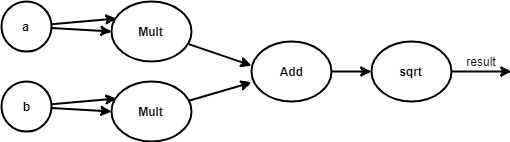
\includegraphics[scale=0.7]{figures/dataflowExample}
\caption{ Pythagorean equation as a Dataflow graph}
\end{figure}

It is easy to infer that a model with such characteristics is ideal for systems with no shared-memory (e.g. distributed systems). A dataflow graph can easily be partitioned into multiple subgraphs, which can then be deployed in any number of different and potentially heterogeneous machines that belong in a cluster, and get executed simultaneously. The problem of transferring data between nodes that have resided on different machines, can be easily treated by serializing them and transmitting them over the network.
There is no doubt why people, in domains that deal with massive data processing, are highly interested in the parallelism opportunities that this model unlocks for them. \\
\linebreak\linebreak\linebreak\linebreak\linebreak\linebreak


    \section{Dynamic Control Flow in Dataflow Systems}
It is highly desirable, as a feature for every dataflow-based system, to be able to embed dynamic control flow constructs inside the dataflow graphs and have an execution model  that  can handle them at runtime \cite{Yu:2018}. The alternative to this, is an “out of graph”, client-side approach which will be better explained below.

    \subsection{Out-of-Graph vs In-Graph Approach}
Current dataflow-based frameworks, allow their clients to specify their desired computations as dataflow graphs via their APIs and provide an execution engine as well, in order to run them. The “out of graph” approach, meets the client’s requirements for expressing dynamic control flow constructs (e.g. while loops) by using the dynamic control flow support of the given client-side language. That means, that, if the framework’s API is accessible via a common, imperative language such as Python, then the client may construct a dataflow graph that corresponds to the body of a while loop and depend on the underlying python execution engine, to run repeatedly the API command that triggers the execution of the graph by the framework’s dataflow executor. This approach, of course, has some disadvantages, as it does not exploit the fact, that the graph has already travelled once, all the way, from the core’s surface to the execution engine, and has already been under many optimization or initialization processes that can be useful throughout all the iteration steps of the while loop.
Some known frameworks that follow this approach are  PyTorch \cite{Paszke2017} or DyNet  \cite{ Neubig2017DyNetTD}.

In-graph approach suggests that the dynamic control flow constructs are embedded inside the dataflow graphs. That means, that the dataflow executor is responsible for managing all the iteration steps of the while loop as well as the logistics that will, eventually, decide its termination, without the intervention of the client’s underlying execution engine.
This approach might be harder to implement but is generally favored due to its noticeably better performance.  \cite{Yu:2018} Having an execution engine that is internally equipped to undesrtand all the characteristics of an iterative construct can be exploited in order to create, initialize, prune and optimize only once the subgraphs that correspond to the bodies of  the while loops during the overall execution which can relieve us from a great overhead.

    \subsection{Dynamic vs Static Dataflow Graphs}
Those who might consider integrating an “in-graph” approach in a dataflow-based system, must concern themselves with two critical matters. First, they need to figure out a way to depict the dynamic control flow constructs in the graph, during its creation. Then, they must ensure that  the system’s execution engine has internal knowledge regarding the operators' semantics and is properly equipped to handle that graph during its execution.

There are two discrete ways that are being followed by various, modern dataflow systems for embedding dynamic control flow inside dataflow graphs, as mentioned in the previous sections. 

First one suggests, that inside the graphs created by the client, any dynamic control flow construct is represented as a node whose operation is rather complex compared to all the other primitive operations. Such nodes are responsible for transforming or/and expanding the dataflow graphs at runtime which is the only period when the dynamic control flow decisions (logistics) can be actually resolved. They are, essentially, copying or adding the demanded subgraphs to the main graph the moment it is clear that they need to be (re-) computed. We refer to every such graph that is subject to transformations at runtime, as "dynamic" graph.  For example, conditional execution would be depicted inside a dynamic graph as a special node which chooses, when gets triggered, to replace itself with the body-subgraph of the corresponding taken-branch (Figure \textit{\textbf{2.2}}).
Note that, in this particular approach, graphs do not contain cycles, as a cycle is nothing but an edge leading back to an already computed subgraph re-triggering its execution. In this solution, every node executes only once. 

The second approach, results in the creation of static dataflow graphs whose form will not be changed by any special, non-primitive nodes during the execution. Any set of nodes corresponding to the body of a while-loop, the body of a recursive function or the bodies of an if-else’s branches, is now integrated in the graphs along with an additional set of primitive operators that constitutes the tagging mechanism that will ensure the correct flow of execution. The notion of “tags”, as will be mentioned below, serves as a way for specifying the context under which every node/operator is executed in cases when multiple instances of it might co-exist at runtime. Contrary to the previous approach, this one allows the creation of cycles as there would be no other way, to express the need for re-computing a certain subgraph in an environment where graphs remain static. 

\begin{figure}
\centering
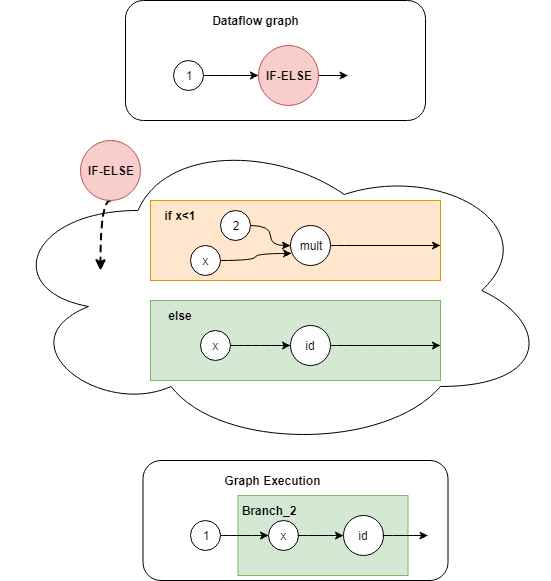
\includegraphics[scale=0.69]{figures/ifelse}
\caption{ Conditional Execution in dynamic approach}
\end{figure}


    \subsection{Recursion in Tagged-Dataflow}

In the conventional, von Neumann architecture, memory (stack) gradually expands during the execution and the data stored in there is mutable (side effects). 
Every time a  recursive function calls itself it initiates the creation of an activation record (frame) which is “pushed” in stack and holds all the data that are local to that specific call (and thus “related” to each other), together. Code is executed sequentially, which causes memory to expand linearly and that is what truly allows the isolation of the data which is critical for avoiding mixing up variables that were derived by different function calls during the computations.

Dataflow's execution model allows the instructions to be executed out of order and in parallel. The next set of operations that are to be executed, at any given moment, comprises those that have all their inputs available, that is, nodes whose incoming edges have all received data generated by the computation of previous operations. In such a model, we have neither stack-behaved memory nor side effects (all data is immutable) as every “variable” is instantly propagated to all the operations that depend on its current value, eliminating the need for a stateful environment.  Representing recursive function definitions (or any dynamic control flow feature for that matter) in static, non-transforming dataflow graphs and executing them cannot be treated the same way now.
If a subgraph (set of nodes), inside the dataflow graph, represents the computations that compose the function’s body, then, intuitively, we would expect that one or more of those nodes (depending on the number of different locations from which this recursive function calls itself) would send their output to the subgraph itself, creating a graph cycle, so that they can possibly re-trigger its execution. What happens though, when we have more than one calls of the same function, executing concurrently?  We have multiple instances of the same operations, awaiting to be triggered by the arrival of data, at the same time. Nothing can guarantee, in this scenario, that an operation instance won’t be triggered by the arrival of data derived by different function calls, hence, the correct execution cannot be ensured and the given results cannot be trusted.

While classic model is gracefully/naturally treating this problem by exploiting the linear memory expansion and making data of the same function calls reside on the same, confined memory locations, dataflow cannot follow, of course, the exact same approach. The equivalent of that solution, would be, to make the flowing data itself hold a piece of information that would indicate the function call from which they were derived. That piece of information is called “tag” in the dataflow community \cite{Nikhil:2000}, and is introduced as the means for overcoming the difficulties described above.\\
 The tag can be anything one desires, as long as it can uniquely “paint” the data, based on the context under which they were derived. 
Now,  in tagged dataflow , the execution of a node will take place, only the moment when all its incoming edges have received data that belong in the same context.
    
\chapter{TENSORFLOW}

TensorFlow  \cite{Abadi:2016} is a rapidly-growing, open-sourced project that is mainly introduced as a system for large-scale machine learning. It is based on the dataflow computational model, which unlocks high parallelism and distribution opportunities and makes it an ideal framework for domains that deal with complex and costly mathematical computations, in general. It was created by Google Brain Team’s researchers and it is now being receiving contributions from all over the world. 

It is one of the numerous \cite{Zaharia:2012,Rossbach:2013, Theano, Jia2014caffe} dataflow-based systems, created by the Machine Learning and Big Data communities, where they are in great need for new, sophisticated frameworks, that will allow them to fully exploit all of their resources in order to process huge amount of data in a reasonable amount of time.

TensorFlow is, basically, a library, whose API allows the users to represent their desired computations as dataflow graphs and set up their execution. 
They are able to configure the cluster on which a graph will be deployed, specify any node placement constraints that will affect the graph's partitioning, select the graph-optimizations that will be, eventually, applied and choose between many more useful setting options.

TensorFlow can run on multiple CPUs and GPUs composing a cluster. That allows users to exploit all of their computational units and deploy on GPUs computations that are complex and better suited to be processed there.

    \section{TensorFlow's Execution Model}

After the client constructs the dataflow graph and initiates its execution, the graph gets pruned so that all the unecessary graph components that do not contribute to the general computation get removed (that is redundant nodes that will never be executed). Then, the resulting subgraph gets optimized by undergoing several transformation procedures and gets partitioned, so that it can be deployed on multiple devices including CPUs, GPUs, or TPUs which are application-specific processing units dedicated to TensorFlow. TensorFlow's execution engine in handling every partition by decomposing it into operations and placing those that are eligible for immediate execution in a ready queue. Every pending operator that is waiting for its input dependencies to be resolved, is placed in the "waiting" queue for future processing. Whenever an operator receives an input generated by the computation of another operator it (re-) examines whether or not it is eligible for execution and it resides on the "ready" or the "waiting" queue, respectively. For the termination of the overall computation to take place, there must be no pending operators inside the waiting and ready queues.
In distributed runtime, there is a main process called "master" that handles the graph's processing before its final execution. Master is aware of all the devices that are available inside the cluster 
and  applies a node-placement algorithm to the graph which places each of its nodes to one such device. Then, it partitions the overall graph with respect to those placement choices and it sends the generated subgraphs to the workers that run on the corresponding machines. Workers are responsible for executing the operators of the subgraph they 've been given and communicate with each other and with the master (who also gets assigned to a subgraph and participates in the execution) in order to transfer their generated data. For the transmission of data  between different tasks/processes TensorFlow uses multiple protocols suitable for every situation depending on whether the tasks run on the same machine or on seperate ones.

    \section{Iteration and Conditional Execution in TensorFlow}
Google favors the in-graph approach for integrating dynamic control flow features in TensorFlow and argues that this implementation yields much better performance results compared to the alternative, mainly because it enables the performing of whole-graph optimizations. \cite{Yu:2018} In addition to that, they have chosen to implement the iteration and if-else features by following the "static" approach that was described before. That means, that they are embedding while-loops and if-else constructs inside non-transforming, static graphs and have created a special set of primitive operators that will ensure the correct flow of execution.

These operators, as well as their semantics, are described below:

\begin{figure}
\centering
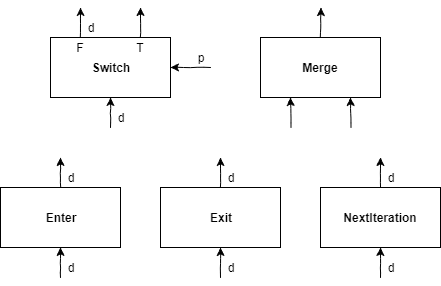
\includegraphics[scale=0.75]{figures/TFoperators}
\caption{ Dynamic Control Flow Operators in TensorFlow}
\end{figure}


    \begin{itemize}

    \item \textit{\textbf{Enter:}} TensorFlow introduces the concept of "frames", which is nothing but a way for describing the context under which a set of computations, composing the body of an iterative construct, will actually take place. Frames are groups of node-instances that are identified by the same shared tag and execute only once under that context. Enter is, essentially, a context-switching operator that forwards its input to a child frame. It is possible that more than one Enter operators may send their inputs to the same frame and in that case only the first one will take the responsibility of creating and initializing it.
\begin{lstlisting}
Eval(Enter(d, name), c) = r, where
	r = (value(d), is_dead(d), tag(d)/name/0)
\end{lstlisting}

    \item \textit{\textbf{NextIteration:}} It is there to create the graph-cycle needed in iteration, in order to express the re-triggering of a while-body's execution. It is similar to the Enter operator, as it also forwards its input to a new, uniquely identified context. Their difference essentialy lies in the way those two operators update the tags of their inputs.
\begin{lstlisting}
Eval(NextIteration(d), c) = r, where
	tag(d) = tag1/name/n
	r = (value(d), is_dead(d), tag1/name/(n+1))
\end{lstlisting}

\begin{figure}
\centering
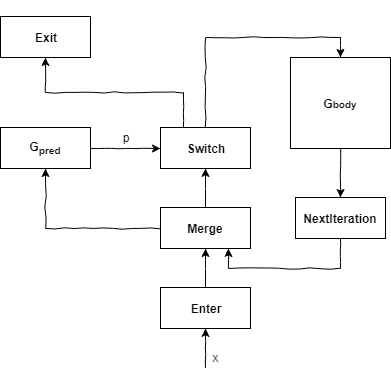
\includegraphics[scale=0.5]{figures/while}
\caption{ Dataflow graph for a while loop in TensorFlow}
\end{figure}

    \item \textit{\textbf{Exit:}} It  is responsible for revoking the actions of the corresponding Enter operator, by forwarding its input to the outer-frame.
 Again, multiple "Exit" operators may exist inside the current-frame, so the last of them that is being triggered is also taking the responsibility of destroying the frame in which it belongs.
\begin{lstlisting}
Eval(Exit(d, name), c) = r, where
	r = (value(d), is_dead(d), c.parent.tag)
\end{lstlisting}

    \item \textit{\textbf{Switch:}} It is used for the representation of if-else constructs and it's job is to "direct" the execution to the correct branch. It receives two inputs of which the first one is the data that needs to be propagated to the correct subgraph and the second one is the result of the computed if-else logistics  (predicate). Depending on the predicate's truth value the switch operator sends the data to either its first or its second output. 

In fact, for reasons that concern the support of distributed execution and will be better explained in the following sections,  the data is actually being sent to both branches, equally, 
except that, the correct output is forwarding the propagated data as "alive" and the wrong one as "dead", which is a phenomenon inofficially described as "deadness propagation".
\begin{lstlisting}
Eval(Switch(p, d), c) = (r1, r2), where
	r1 = (value(d), p || is_dead(d), tag(d))
	r2 = (value(d), !p || is_dead(d), tag(d))
\end{lstlisting}


    \item \textit{\textbf{Merge:}} It goes as a pair with the Switch operator and is added to the place where the two branches join, in order to collect the if-else' s generated output. It expects two inputs, of which only one will be valid and forwarded, the one generated by the taken-branch. Merge operator, however, is playing another, significant role in the representation of iterative constructs, i.e. while loops. It is placed as a successor to all the existing Enter/NextIteration operators, so that it can distinguish between the first time we execute the body of a while loop and all the following ones. That is, so that  it will always provide the correct input to the while's body-subgraph. 
\begin{lstlisting}
Eval(Merge(d1, d2), c) = r, where
	r = if is_dead(d1) then d2 else d1
\end{lstlisting}

    \end{itemize}



Figures \textit{\textbf{3.1}} and \textit{\textbf{3.2}}  can be found in the "Dynamic Control Flow in Large-Scale Machine Learning" paper  \cite{Yu:2018} where the dynamic control flow support in TensorFlow is being discussed in much more detail. 

\section{Recursion in TensorFlow}
As for the case of recursion, TensorFlow's support is still at a rudimentary level. They built a way for allowing users to define recursive function definitions via the python API,  and supported it up until their r.1.4 TensorFlow release. They removed it, however, later on, (possibly termporarily) due to conflicts occured in their future development. Contrary to the other two dynamic control flow features, Google chooses to support functions and thus, recursion, by following the "dynamic approach".  They have created an operator named "Call", that is placed as a node inside the graph and represents the calling of a function. Every such node contains important information that associates it with the definition  of the function that is being called.  "Call" node's job is, essentially,  to replace itself with the body of that function, causing the dynamic expansion of the graph, as many times as needed. The real implementation might be a slight derivation of what was described above but the essence of the approach is exactly the same.

The main disadvantage of this particular approach, has been already discussed in the "Motivation" subsection.

\begin{flushleft}
  In figure 3.4, we present an example of calling functions, expressed as a functional program and the way it will be converted into a dataflow graph and get executed in TensorFlow:

 \setlength{\parindent}{25ex} $result = f(4) + f(5)$ \\
$f(x) = g(x+1)$ \\ 
$g(y) = y$
\end{flushleft}

The equivalent example, expressed in TensorFlow via the Python API is also presented below:
\begin{lstlisting}
import tensorflow as tf
from tensorflow.python.framework import function

@function.Defun(tf.int32)
def G(y):
	return y

@function.Defun(tf.int32)
def MyFunc(x):
	return G(x+1)

a = tf.constant(4)
b = tf.constant(5)

result = MyFunc(a) + MyFunc(b)

with tf.Session() as sess:
	print(sess.run(result))
\end{lstlisting}

\begin{figure}
\centering
\includegraphics[scale=0.6]{figures/Tf_recursion}
\caption{ Calling functions in TensorFlow}
\end{figure}


\chapter{APPROACH}

    \section{Tagging in Recursion}

As already mentioned before, integrating the static approach requires employing a tagging mechanism that will solve the problem of potentially mixed-up data, in cases when multiple instances of same operations are being executed simultaneously (overlapping recursive function calls or iterations).

Iteration and recursion are nothing but two different mechanisms for triggering the repetitive execution of a certain code-segment (here subgraph). One can say that the first one is, essentially, a subset of the second one, as every possible iteration-loop can be expressed as a tail recursive function. 

In the dynamic approach, we would expect that an iterative construct would trigger the linear expansion of the graph, whereas, some recursive ones, would cause the graph to expand in a tree-like way. That said, we can now have a sense, perhaps, of how the tag, in each case, must be represented. 

Non-formally speaking, in the simple case of one  loop, we have multiple instances of the same subgraph (loop’s body) firing whenever they are triggered, and creating a "chain" as the loop keeps unfolding. In that case, a simple number belonging in the set of natural numbers would suffice as a tag that would make one chain piece distinguishable from the others. However, if we are able, at each given moment, to trigger the simultaneous execution of that particular subgraph an arbitrary amount of times by different call sites, as happens with recursion, that representation would not be satisfactory. Intuitively we would need a more profound way to capture the topological position of each subgraph-instance inside the resulting “function-calls tree” and that would be by using lists of natural numbers with unspecified length.

    \section{Yaghi's Transformation}
The problem of how recursion can be expressed in static dataflow graphs and the tagging mechanism that needs to be employed in order to track the depth and path of each recursive function call, has already been resolved in past research work and a formal basis for the aforementioned matters has already been provided.  \cite{Rondogiannis:1997}

There has been described a systematic way for producing static dataflow graphs from potentially recursive function definitions based on an algorithm called “Yaghi’s transformation”, proposed by A. Yaghi as a subject for his PhD dissertation, in 1984.

This algorithm provides a method for transforming first-order functional programs into intentional ones which, as the conducted research suggests, can be easily deployed and executed in dataflow architectures running a demand-driven computational model, called Eduction.

Yaghi, also, introduces two new operations named \textbf{calli} and \textbf{actuals} which can be  thought of as two common, context-switching operators. 
The description of their semantics can be found in this paper \cite{Rondogiannis:1997} in a very formal and detailed way and we urge the reader to look there for acquiring a better understanding of Yaghi's transformation.\\

Yaghi's algorithm consists of three steps which are summirized in the paper, as follows:

    \begin{itemize}
    \item Let \textbf{f} be a function defined in the source functional program. Number the textual ocurrences of calls to \textbf{f} in the program, starting at 0 (including calls in the body of the definition of \textbf{f}).
   
   \item Replace the ith call of \textbf{f} in the program by \textbf{calli(f)}. Remove the formal parameters from the definition of \textbf{f}, so that \textbf{f} is defined as an ordinary individual variable.
   
   \item Introduce a new definition for each formal parameter of \textbf{f}. The right hand side of the definition is the operator \textbf{actuals} applied to a list of the actual parameters corresponding to the formal parameter in question, listed in the order in which the calls are numbered.
    \end{itemize}


\begin{flushleft}
If we apply these steps to this functional program:\\
 \setlength{\parindent}{25ex} $result = f(4) + f(5)$ \\
$f(x) = g(x+1)$ \\ 
$g(y) = y$
\end{flushleft}

\begin{flushleft}
we end up with its corresponding intensional one:\\
 \setlength{\parindent}{25ex} $result = call_0(f) + call_1(f)$ \\
$f = call_0(g)$ \\ 
$g = y$ \\
$x = actuals(4,5)$ \\
$y = actuals(x+1)$ \\
\end{flushleft}

Informally speaking, when \textbf{calli(f)} gets evaluated under a context c, where c is  a list, it augments the list by prefixing it with i and it returns f's value under that new context.  On the other hand, when \textbf{actuals} gets evaluated under a context c, where c is a list of  integers whose head is i, it returns its  i-th argument. Again, however, resorting to the paper is necessary in order to fully comprehend the way they operate as well as the intuition that lies behind their semantics.

\begin{flushleft}
The intensional program can be easily executed by an eductive computational model, as follows:\\
 \setlength{\parindent}{15ex} $EVAL(call_0(f)+call_1(f), [])$ \\
$EVAL(call_0(f), []) + EVAL(call_1(f), []) =$ \\ 
$EVAL(f, [0]) + EVAL(f, [1]) =$ \\ 
$EVAL(call_0(g), [0]) + EVAL(call_0(g), [1]) =$ \\ 
$EVAL(g, [0,0]) + EVAL(g, [0,1]) =$ \\ 
$EVAL(y, [0,0]) + EVAL(y, [0,1]) =$ \\ 
$EVAL(actuals(x+1), [0,0]) + EVAL(actuals(x+1), [0,1]) =$ \\ 
$EVAL(x+1, [0]) + EVAL(x+1, [1]) =$ \\ 
$EVAL(x, [0]) + EVAL(1, [0]) + EVAL(x, [1]) + EVAL(1, [1]) =$ \\ 
$EVAL(x, [0]) + 1 + EVAL(x, [1]) + 1 =$ \\
$EVAL(actuals(4,5), [0]) + 1 + EVAL(actuals(4,5), [1]) + 1 =$ \\
$EVAL(4, []) + 1 + EVAL(5, []) + 1 =$ \\
$4+1+5+ ) =$ \\
$11$ \\
\end{flushleft}


The above work introduces the idea of expressing tags as integer-lists of arbitrary length and essentially describes the additional, primitive, context switching operators that implement the tagging mechanism we need for the static approach. Applying the ideas that were expressed in that research to dataflow systems that run a data-driven execution model was rather easy, but a formal, theoretical proof of the data-driven “version” should, definitely, be provided.

    \section{Basic Idea}
We can resolve the problem of integrating recursion in dataflow-based systems, without allowing any graph-transformations at runtime ("static" approach), by first addressing the following critical matters.

We, first, need to establish a way for representing recursive function definitions as dataflow graphs.  That can be easily treated, as already mentioned before, by allowing the occurence of cycles inside those graphs. If a subgraph (set of nodes), represents the computations that compose the body of a function, then we represent a recursive call to that function by creating a cycle between the node that corresponds to the call site and the subgraph itself. That edge unlocks the possibility of  re-triggering the subgraph's computation and thus, re-executing the function as many times as needed, without dynamically transforming the main executable graph.

Then, we must ensure that, if a function is being called, at least once, inside the program, then the subgraph that constitutes the representation of that function will have to be statically integrated in the main subgraph. Every call to that function from the outer-main graph, will be represented from now on, as an edge, connecting the node that corresponds to the call site to the entering point of the callee function/subgraph.

The form of the resulting graph, however, is not complete yet. We also have to specify an additional set of two primitive operators that will constitute the tagging mechanism that needs to be employed. These operators will also be added to the graph and will ensure the correct flow of execution.

We call these two operators "Call" and "Return" and their function is to guard the entrance/exit of the data to/from the function's scope, respectively.

    \begin{itemize}

    \item \textit{\textbf{Call:}} This operator is placed as a guard to all the entry points that lead to the body of a function. It receives, as input, the function's arguments, as those are yielded by the caller and it updates their tags appropriately, before forwarding them to the correct function nodes. This generated tag will make uniquely identified, at runtime, that specific function instance and will constitute the context under which all the entering data will eventually be executed. This ensures that data derived by different, overlapping calls to the same function won't get mixed up during the execution.

    \item \textit{\textbf{Return:}} This operator is placed as a guard to all the function's exit points. It receives, as input, data generated by the "returning nodes" of that function (function's outputs) and it updates their tags appropriately, before forwarding them to the caller (outer-graph).  The "Return" operator updates the tag by revoking the changes the corresponding "Call" operator previously made, retrieving that way the correct "parent-context".

    \end{itemize}

All the different call-sites from where all the possible function calls may occur at runtime, are statically depicted in the initial graph and therefore, can be enumarated.
Every such call-site is uniquely associated to a specific pair of "Call/Return" operators. These operators keep internally stored the call-site's numbering and they will use that information, at runtime, for creating globally unique tags. 

\begin{figure}
\centering
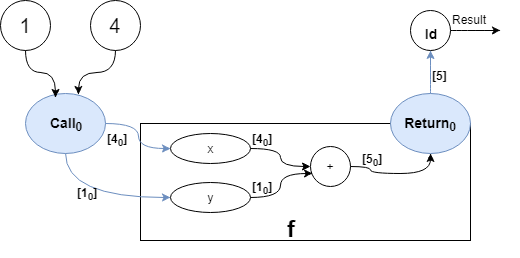
\includegraphics[scale=0.65]{figures/Example1}
\caption{One call to a simple, non-recursive function}
\end{figure}

For reasons we mentioned again earlier, tag could be an integer-list of unspecified length. This representation is satisfactory for tracking the depth and path of all the (potentially recursive) function calls.

In the simple example, presented in \textit{\textbf{Figure 3.1}}, function \textit{\textbf{f}} is being called only once, from the main graph. We have one call-site numbered with 0. The corresponding "Call/Return" pair has internally stored that number. "Call" operator tags with it its incoming data, and "Return" operator extracts it from its input's tag. 

Everything works fine in this scenario, but what happens when we have more than one calls to the same function? 
The "returning node" (+) of function  \textit{\textbf{f}} is connected to  two different "Return" operators, as shown in \textit{\textbf{Figure 3.2}} and must decide, each time,  where is the correct place to send its generated output.

For treating this problem, we are extending the way the "Return" operator functions.  Function \textit{\textbf{f}}'s returning node will  propagate its data to every possible "Return" operator that lives inside the body of all the potential callers and a "Return" operator will operate on an incoming input only if it decides that the input's tag concerns it.

That said, we can now be more specific about the semantics of  "Call" and "Return" operators and the way they update the tags of their inputs:
    \begin{itemize}
    \item \textit{\textbf{Call }} operator appends its internally stored number to the list/tag of its input and then forwards that input to its corresponding output. The generated tag is guaranteed to be globally unique.
    \item \textit{\textbf{Return }} operator examines the last element (integer) of its input's list/tag. If it matches its internally stored number, it officialy extracts it from the tag and forwards the input to its output. If not,  it performs no further actions.
    \end{itemize}

Note that, the dataflow graph in \textit{\textbf{Figure 3.2}} is still incomplete, as it needs an additional operator that will help distinguish between the inputs provided by the different calls. The classic "Merge" operator whose semantics are described in the majority of  the existing "dataflow" papers (it was also mentioned in the "Dynamic Control Flow in TensorFlow" subsection as it is used in TensorFlow, too), is ideal for this job. It is placed as a successor to all the "Call" operators and it chooses, each time, to accept only one input.

Note also, that everything discussed above, applies to cases where we have mutually recursive function calls, too. 

\begin{figure}
\centering
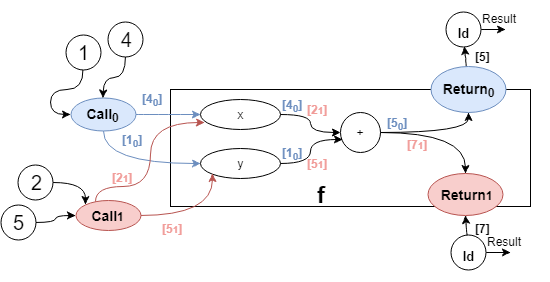
\includegraphics[scale=0.7]{figures/Example2}
\caption{Two calls to a simple, non-recursive function}
\end{figure}

In  \textit{\textbf{Figure 3.3}}, we present a more complex and interesting example of the case we are more concerned with in this particular project. That is, recursion. The example depicts the dataflow graph of a simple program where  \textit{\textbf{factorial}} gets called once.

\begin{figure}
\centering
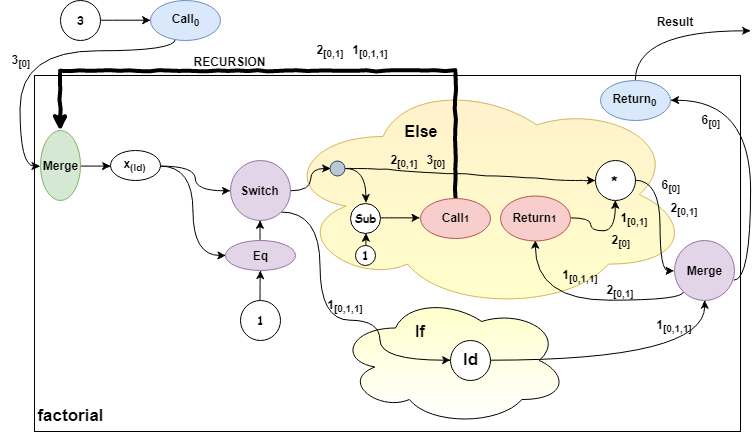
\includegraphics[scale=0.65]{figures/factorial}
\caption{Factorial}
\end{figure}

\chapter{IMPLEMENTATION}
In the previous section, our aim was to provide a more general and abstract description of the "static" approach and to present the fundamental basis of our implementation so that it can be, theoretically, applied to all the existing dataflow frameworks. 

In this section, however, we present all the technical details that concern the integration of that approach in TensorFlow's infrastructrure.

Our main goal was to integrate our implementation as an additional feature to the framework. That means that we did not perform any changes to Google's already existing code but we, instead, built on top of it so that we can provide an additional method for representing and executing functions, in general. Clients can deliberately choose, via the API, whether they want to apply our approach or ignore it completely in which case Google's default way for supporting functions will prevail.

We chose to base our implementation on TensorFlow's r.1.4 release in which the definition of recursive functions via the Python API was still supported. That way we could relieve ourselves from all the dirty, interface-related details and make the most out of exploiting TensorFlow's existing infrastructure.  



    \section{Graph Transformation}

TensorFlow is an extremely flexible framework that  can be easily extended by the users, so that they can perform their own experiments on it. People may want to implement and test their  ideas either for improving the framework's performance or for research purposes, in general. For that, they are allowed to define their own graph-optimization techniques, implement better node placement algorithms, create new additional operators or even add their own, personal execution engines (executors).

Once a dataflow graph is constructed, it passes through a number of different stages before it is ready for execution. One such stage is where it undergoes many transformation procedures that are meant to optimize its form. We managed to add a new optimization algorithm, called "function-transformation", that takes place before the graph's partitioning and changes its form, in case it detects any function-call occurences.
As already mentioned before, TensorFlow's  way of dealing with functions and thus, recursion is based on the "dynamic" approach. That means that every function call is represented, inside the main graph, with a special node, whose job, when it gets executed, is to replace itself with the body of that function. The "function-transformation" algorithm  manages to transform this specific representation to the one we want and described in the "Approach" section. 

As shown in \textit{\textbf{Figure 4.1}}, when this algorithm detects a special node calling a function, it replaces it with a new pair of "Call/Return" operators whose semantics are identical to those we described above. The algorithm must ensure that the bodies of all the callee functions are embedded inside the graph at least once (inlining).
When a "Call/Return" pair takes the place of a special node, we must attach all the incoming edges of that node to the inputs of the "Call" operator. Respectively, all the outgoing edges of that node will constitute the outputs of the corresponding "Return" operator. Function transformation also adds the "Merge" operators that are needed in case we might have multiple calls to the same function, from different call-sites. It places them between the "Call" operators and the nodes that expect the arguments of the function, for reasons already mentioned.

\begin{figure}
\centering
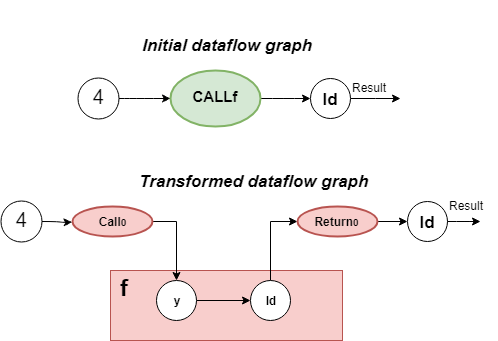
\includegraphics[scale=0.65]{figures/transformation}
\caption{Function Transformation}
\end{figure}

Every "Call" operator, as described until now, must first gather all the function's arguments before propagating them to the nodes that need them inside the body of that function. Respectively, "Return" operator is waiting to gather all the function's returning nodes before propagating them to the outer-graph. This is, however, a limiting factor for the potential parallelism that can be achieved. Similar to what Google already does for the "Enter/Exit" operators to cure this problem, we break every "Call" and "Return" operator into multiple ones, with each one of them corresponding to a single/unique function argument/returning node. That way we can increase the number of overlapping function calls, during the execution.


In  \textit{\textbf{Figure 4.2}} we present the dataflow graphs of a simple program where \textit{\textbf{factorial}} gets called once, as generated by TensorBoard. 
The graph on the left is the one generated after the "function-transformation" took place, whereas the one on the right is the initial graph generated by Google's "dynamic" approach.
If we click and extend, in TensorBoard, the red "Fac" (Factorial) box that's inside the graph on the right, another identical copy of the Factorial will be revealed and that could go on, endlessly.

TensorBoard is a visualization tool, built by Google. It has several utilities but we used it extensively for visualizing the generated TensorFlow graphs which was extremely helpful for studying them and debugging our code.\\\\\\\\\\\\\\\\\\\\\\\\

\begin{figure}
\centering
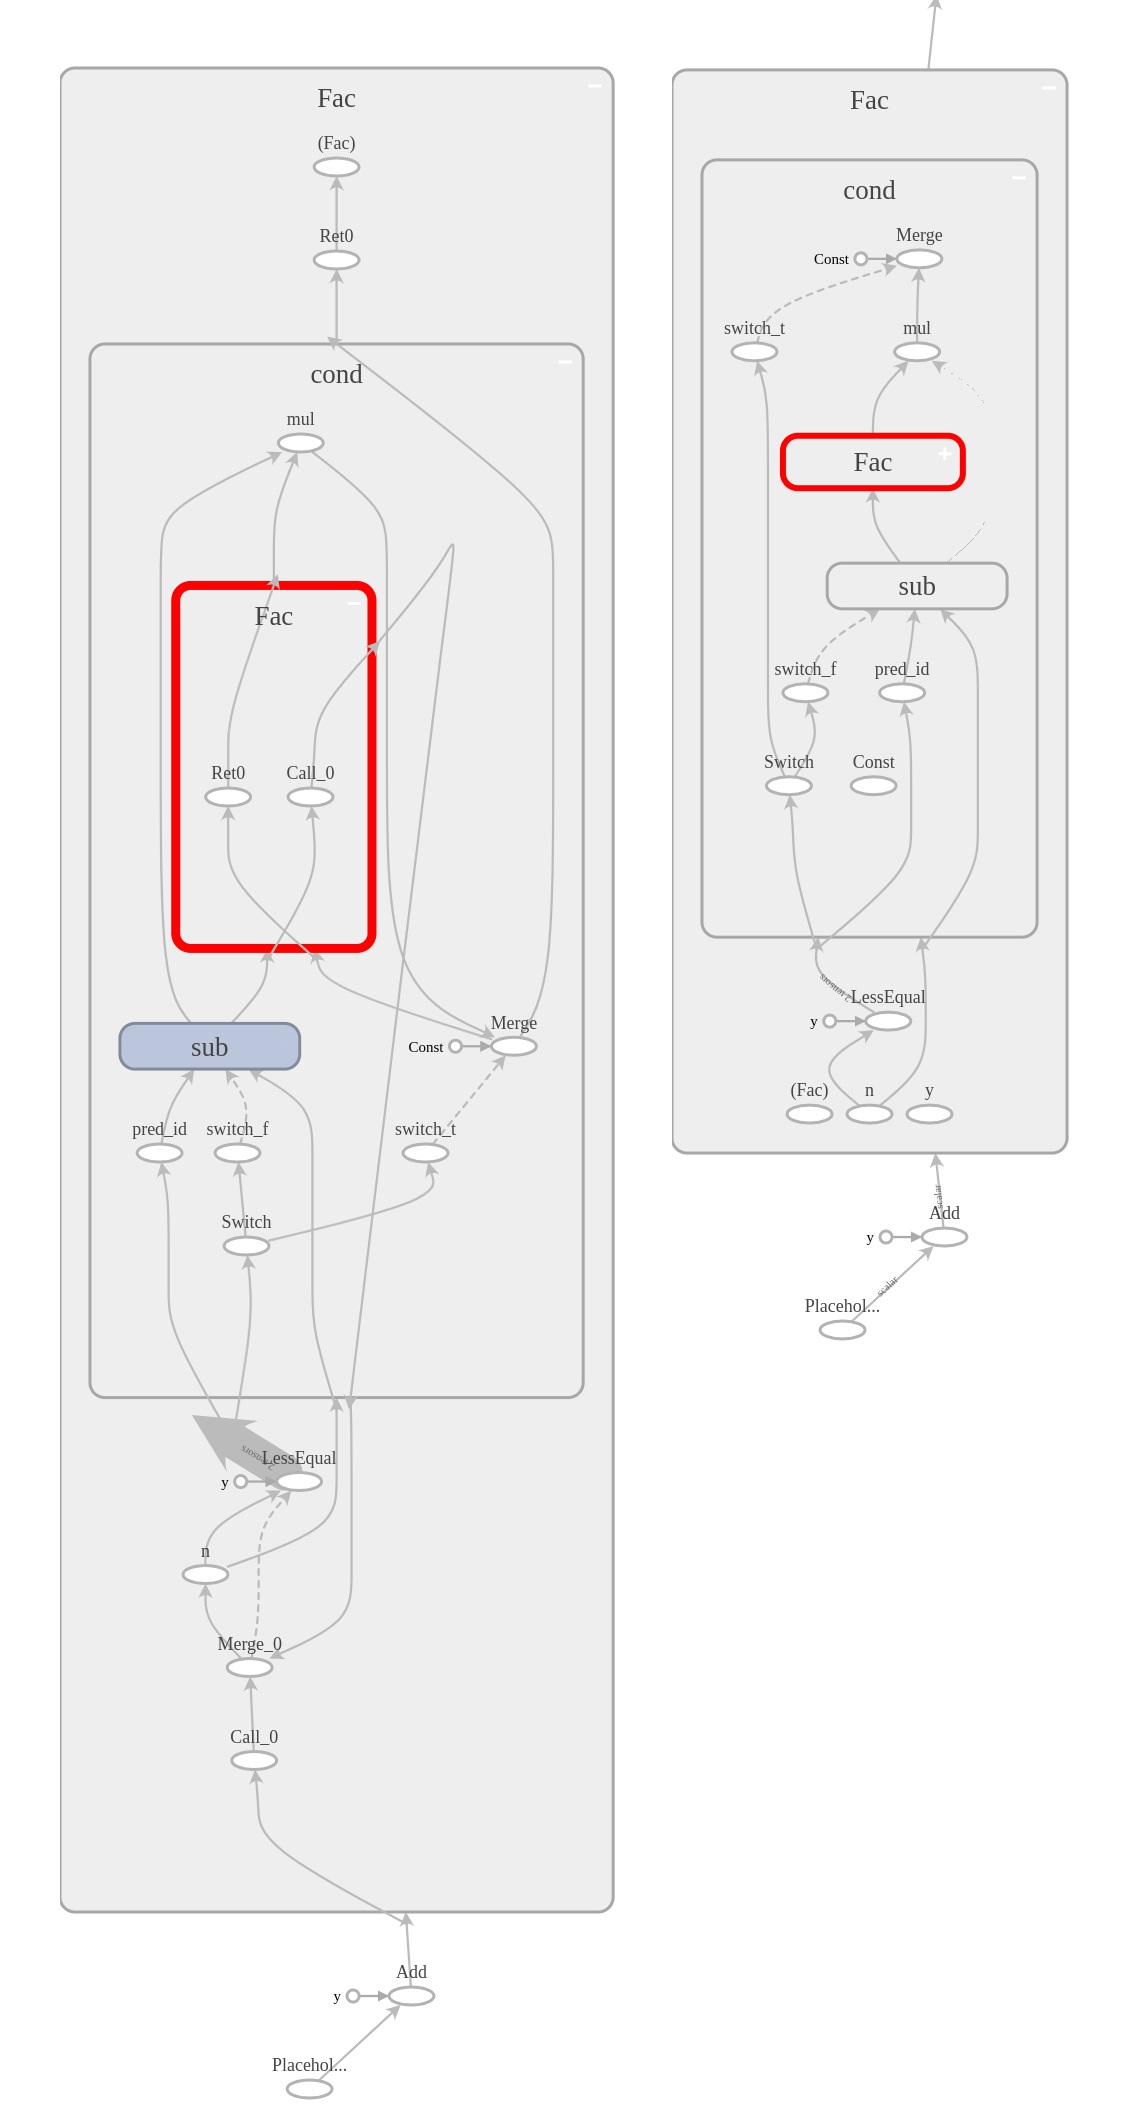
\includegraphics[scale=0.42]{figures/tf_factorial}
\caption{TensorFlow graphs for factorial in "static" and "dynamic" approach}
\end{figure}



    \section{Local Execution}


After succesfully transforming the graph, its resulting form can gracefully capture and depict in its entirety, every possible recursive mechanism defined by the client, in a way that relieves us from the need of using non-primitive, special operators with such costly and complex kernels. We, essentially,  eliminate every such special node as well as the additional overhead that it imposes by replacing it with two other, less costly, primitive operators (Call/Return) that only forward their inputs and manage frames.  The overhead added by the management of tags is not insignificant either, but with the appliance of the appropriate optimization techniques it can be limited significantly.

Of course, our work doesn't end with the transformation. We may have succeeded so far, in ending up with representations that favor the "static" approach but we haven't ensured, yet, that the  execution engine recognizes the introduced operators and thus, understands how to properly treat the graph at runtime. Consequently, the next matter we needed to attend to was the registration of the Call/Return operators and the implementation of their kernels.  For the sake of consistency, we tried to do that by constantly consulting Google's pre-existing code for iteration, as Call and Return operators do not differ from Enter and Exit that much, after all. In fact, one can say that the first two are nothing but a generalization of the second ones. 


As a continuation to Google's attempt at describing their operators' semantics, we provide below, in a similar vein, the evaluation rules of our newly introduced operators:

\begin{flushleft}
$Eval(Call(d, name), c) = r,\  where$ \\
\setlength{\parindent}{5ex} $r = (value(d), is\_dead(d), tag(d)/name)$
\end{flushleft}

\begin{flushleft}
$Eval(Return(d, name), c) = r, where \ $ \\
\setlength{\parindent}{5ex} $tag(d) = tag1/name$\\
$ r = (value(d), is\_dead(d), tag1)$
\end{flushleft}

%\begin{flushleft}
\textit{Note that, the evaluation of "Return" is not defined for the case where it receives data that were derived by a call from a different call-site.}\\
%$ Return(d, name), where \ $ \\
%\setlength{\parindent}{5ex} $tag(d) = tag1/name1,$\\ 
%$name \neq name1$
%\end{flushleft}

After registering Call and Return in TensorFlow and making the appropriate adjustments to the execution engine, the semantics of these two operators are now fully conveyed to TensorFlow's infrastructure and the implementation for "local execution" is considered to be complete. From now on, any example of simple or mutual recursion can be executed via the "static" approach, too, if the client chooses so.

Something that should be noted is, that, contrary to the case of iteration, the execution of non-tail recursive functions imposes what might constitute a significant performance issue.
We have no control of parallelism. That is, we cannot impose a limit to how many calls of a recursive function can execute in the machine, at the same time.
Ιt is easy to specify a maximum number of overlapping iteration "steps"  because the execution of an iteration step that exceeds the limit can simply be stalled (TensorFlow does such thing for limiting parallelism). However, in cases where we are dealing with non-tail recursive functions, the execution of one function-call depends on that of another one and those dependencies between parent-children function calls go on until we reach a base case. Therefore, imposing similar parallelism limitations will most probably cause a deadlock.


    \section{Distributed Execution}

Executing graphs without deploying them on clusters is not wise in terms of performance.  Using dataflow systems only for 'local exeuction' not only does not exploit their immense potential  for parallelism/distribution but also yields slower performance results compared to other classic systems, as the overhead that they impose by trying to emulate the dataflow computational model is very significant. 
That is why, implementing a "dynamic control flow" approach that favors the distributed execution is extremely important. 

We already saw that, the resulting graphs in "static" approach contain the bodies of any existing, callee functions. That means that, contrary to TensorFlow's approach, we are now able to include these subgraphs in the partitioning and assign the function nodes to be executed on different machines, in ways that will improve performance the most.

The partitioning of a recursive function definition, however, as well as that of any other dynamic control flow construct  when we follow the "static" approach, is not that easy to perform in TensorFlow.
TensorFlow's design allows the execution of each partition to make progress independently, without conforming to constraints imposed by a centralized coordinator \cite{Yu:2018}. That maximizes the potential for better performance, but makes the partitioning a challenging procedure.

Remember that, in static approach, any subgraph corresponding to the body of a while loop or a recursive function, is provided with a tagging mechanism that will create/destroy frames and produce different contexts under which those computations will take place. This mechanism is nothing but an additional set of primitive, context switching operators which are, also, subject to partitioning. A partition, however, cannot include any partially composed "mechanisms" as this would cause the incorrect generation of frames/tags, inside a machine, during execution. We have to make sure that, every partition that contains nodes that will be executed under different contexts/frames, will also contain all the necessary mechanisms for generating that frames.

In order to add support for distributed execution, in our implementation for recursion, we adopted a similar solution to the one Google already proposes for the case of iteration, yet more generalized. Google's solution keeps track of all the iterative constructs that are embedded in a graph as well as their mechanisms for generating and destroying frames. Whenever a loop is "shared" between multiple partitions, the corresponding mechanism, referred to as control-loop state machine,  will be added to all of them. A simple control-loop state machine consists of an Enter, a NextIteration, a Merge and a Switch operator as shown in  \textit{\textbf{Figure 4.3}} where we present an example also found in the "Dynamic Control Flow in Large-Scale Machine Learning" paper \cite{Yu:2018}.

However, in case of recursion, the form of a "control-recursion" state machine is slightly more complex. Here, we may have multiple conditional branches, with each one of them, leading either to a base case or a simple/mutually recursive call or a simple call to a different possibly recursive function e.t.c. What we do in order to extract the correct form of the state machines in every case, is traversing the graph and capturing all the special operators that constitute the dynamic control flow's backbone as well as the way they are connected to each other. When traversing the graph we ignore common and non context-switching operators as they will neither be included in the eventual state machine nor they will give us important information about the dynamic control flow construct's structure. We take into account the Call, Return, Switch, Merge operators and all of them, with the exception of "Return" nodes, will be added to the state machine that will eventually  be copied to all the appropriate partitions. The way these operators will be connected to each other, inside the state machine, is inferenced during the graph's traversal.

\begin{figure}
\centering
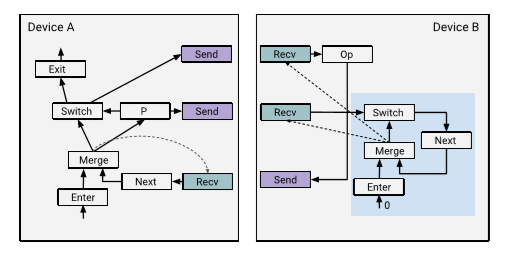
\includegraphics[scale=1.2]{figures/sm_iteration}
\caption{Distributed execution of a while-loop in TensorFlow}
\end{figure}



As shown in \textit{\textbf{Figure 4.3}}, whenever two connected nodes  reside on two different partitions, TensorFlow creates and places between them, two additional special operators that handle the transition of the data via the network. These nodes, named "Send"  and "Receive", get connected to the nodes that send the data and receive it, respectively and each one of them resides on the same partition as its connected node does. 

We already made a reference, in a previous section, to a phenomenon called deadness propagation. In cases where a conditional branch is not taken, the nodes that compose it are being executed anyway. The difference is that these nodes do not perform computations. They are considered to be "dead" and all the outputs they generate are propagated as "dead", too. 
The reason why this is happening, is  because "Receive" operators do not formally have any incoming edges and that makes them qualified for immediate execution. Their computation is terminated the moment they receive data from its corresponding "Send" operators that belong in other partitions. However, there may exist "Receive" operators, that have been triggered to wait for data generated by nodes that belong in non-taken branches. Normally, those operators would block indefinately, as they would never reveive any data, but now, with deadness propagation, they will accept data tokens indicated as dead and their execution will be officially terminated.

In the case we are dealing with, in our implementation, we may have conditional branches that contain simple/mutually recursive calls. The nodes of these branches are  also expected to generate dead data in case the branches are not taken, so we have to ensure somehow, that deadness will manage to get propagated through the callee recursive functions, too. This, however, constitutes an issue, as the recursive "Call" operators might cause the propagation to get caught in an endless loop or freeze in general. We are treating this by inserting a control-edge that directly connects  the "Call" operator to the corresponding "Return". So, now, "Call" manages to propagate deadness immediately through the "Return" operator. 

\textit{Control edges are edges that do not transfer data. They are only added between two nodes in order to impose ordering constraints.}

\begin{figure}
\centering
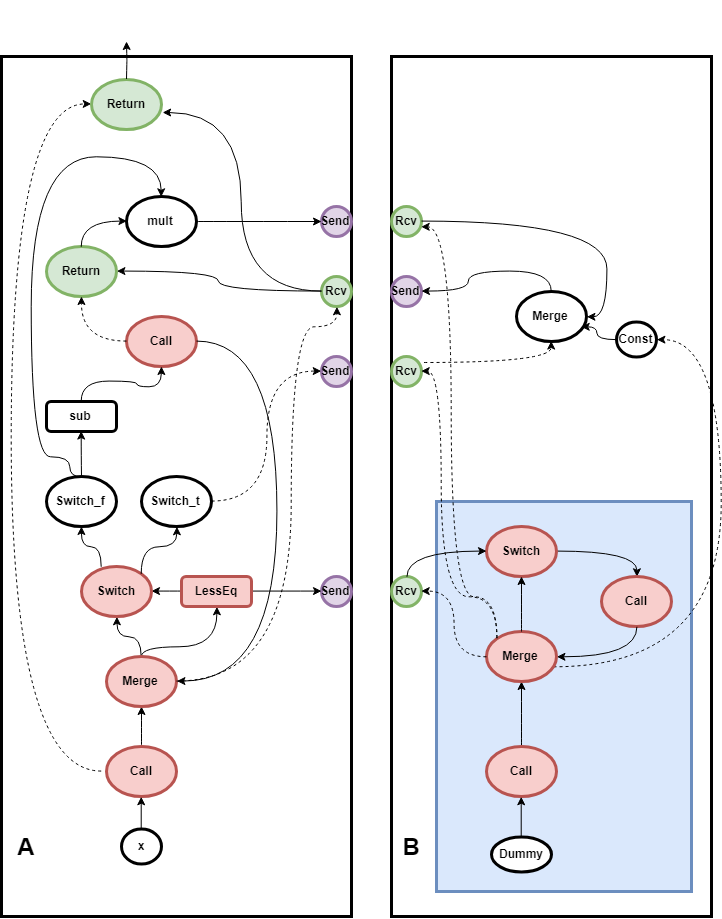
\includegraphics[scale=0.6]{figures/DistrFac}
\caption{Distributed execution of Factorial}
\end{figure}

Note that, \textit{\textbf{Figure 4.4}} is an informal example of factorial graph's partitioning. The formal partitions/graphs, as generated by TensorBoard, are more detailed and contain a lot of dirty information that would only distract the reader from understanding the essence of this example. 

It is obvious that our implementation is a generalized version of Googles'. 

Below, we present some details regarding the partitioning, in the previous example:
    
\begin{itemize}
    \item Every state machine's Merge operator is connected, via control-edges, to all the Receive operators that exist in the same partition, so that it can enable their execution under the correct context/frame.
    \item Every state machine's Switch operator must receive the corresponding "predicate" from the partition that generates it.
    \item Every Call operator has a control-edge directed to its corresponding Return operator, so that it can immediately propagate through it any dead data. Notice that, without this control-edge, the execution of the above example would fail.
    \item State Machine, in partition B, contains a dummy constant that sends output to the Call operator. Its job is to initiate the execution of this Call so that the state machine starts emulating the execution of the recursive function and generating frames.
    \item We like to think of  the state machines as the dynamic control flow construct's backbone. It is the minimum set of special nodes that  is able to emulate the correct generation of frames during execution.
    \end{itemize}



\chapter{RELATED WORK}

 \textcolor{blue}{korean guys\cite{Jeong:2018}}

 \textcolor{blue}{other frameworks}

\chapter{FUTURE WORK}

   \section{Higher Order Functions}

An interesting extension to our work would be to investigate ways of defining higher-order functions in static dataflow graphs, too. That is, functions that may accept other functions as arguments , which can then be called by the first ones. An extension of Yaghi's transformation that partially solves this problem is described in this  \cite{RondogiannisW99} paper, however, this topic needs some more extended research. After establishing a formal, theoretical solution of this matter, those ideas could also be integrated in TensorFlow, in the future.

    \section{Automatic Differentiation}

 \textcolor{blue}{Machine Learning blah blah}


\chapter{EVALUATION}

\chapter{CONCLUSIONS}

The main goal of this project was to apply the ideas expressed in this \cite{Rondogiannis:1997} paper to an existing dataflow-based framework. The reason why TensorFlow was chosen, is because of its rapidly-growing fame and the fact that it is open-sourced. Another important reason is that TensorFlow already follows the static approach for supporting conditional and iterative execution. Yaghi's transformation and the aforementioned research  served as a guide to us, throughout the whole implementation.  However, for the practical part of our work, which was the development,  Google's support for iteration was a significant benchmark. This project can be thought of, perhaps, as an extension of Google's work for supporting dynamic control flow features. The reason why the "static" approach has not been already followed, in TensorFlow, for the support of functions, too,  is more or less a mystery to us.

In this work,  we proposed a systematic way for embedding recursive function definitions in static dataflow graphs. We described the form of these graphs and the additional set of context-switching operators that enable their correct execution. We also presented some of the issues we encountered while implementing everything in TensorFlow, as well as the solutions we came up with in order to overcome these obstacles.

The content of this bachelor thesis is supposed to be more dataflow-oriented. That means that we have not discussed in great detail matters that concern the field of  Machine Learning and this particular aspect of TensorFlow. We treated it as a dataflow framework that serves as a tool for performing  costly, numerical computations, in general. However, TensorFlow was  built as a system for large-scale machine learning and for that reason, our lack of support for the "automatic differentiation" feature, makes this work incomplete. We cannot build examples of recursive neural networks on which we can test our implementation and evaluate it.  Thus, a more formal comparison between our approach and Googles', based on TensorFlow's real-life applications, cannot be provided, within this bachelor thesis.


\backmatter

% abbreviations table
\abbreviations
\begin{center}
	\renewcommand{\arraystretch}{1.5}
	\begin{longtable}{ l @{\qquad} l }
	\toprule
	NKUA    & National and Kapodistrian University of Athens\\
	NCSR-D & National Centre for Scientific Research-Democritos \\
	PC & Program Counter \\
	CPU & Central Processing Unit\\
	GPU & Graphic Processing Unit\\
	TPU & Tensor Processing Unit\\
	\bottomrule
	\end{longtable}
\end{center}

% appendix
%\begin{appendix}
% mark the beginning of the appendix
%\appendixstartedtrue

% add appendix line to ToC
%\phantomsection
%\addcontentsline{toc}{chapter}{APPENDICES}

%\chapter{FIRST APPENDIX}

%\end{appendix}

% manually include the bibliography
\bibliographystyle{plain}
\bibliography{references}
% include it also in ToC (do sth on your own)
\addcontentsline{toc}{chapter}{BIBLIOGRAPHY}

\end{document}
